\section{Experiments}
In order to experiment the proposed method, we first collected a dataset (details in Section~\ref{dataset:sec}). We labelled small part of the dataset with frame-wise activity step labels and used the resulting set as an evaluation corpus. Neither the set of labels, nor the temporal boundaries are exposed to our algorithm since the set-up is completely unsupervised. We evaluate our algorithm against the several unsupervised clustering baselines and state-of-the-art algorithms from video summarization literature which are applicable. 
\subsection{Dataset}
\label{dataset:sec}
We initiate our data collection using WikiHow as obtaining the top100 queries the crowd is interested and choosing the ones which are directly related to the physical world and objects. In other words, we ignore the queries like \emph{How to get over a break up‏?‎} as they have no objective set of steps. Resulting queries are;


\emph{\textbf{How to}}\footnotesize
\emph{Bake Boneless Skinless Chicken, Make Jello Shots, Cook Steak, Bake Chicken Breast, Hard Boil an Egg, Make Yogurt, Make a Milkshake, Make Beef Jerky, Tie a Tie, Clean a Coffee Maker, Make Scrambled Eggs, Broil Steak, Cook an Omelet, Make Ice Cream, Make Pancakes, Remove Gum from Clothes, Unclog a Bathtub Drain}
\normalsize

For each of the queries, we crawled YouTube and got the top 100 videos. We also downloaded the English subtitles if they exist. For evaluation set, we randomly choose 5 videos out of 100 per query. Hence, we have total of 125 evaluation videos and 2375 unlabelled videos. We label the start and end frames of activity steps (\ie based on the steps of the recipe) as well as the name of the step. We will release the code and collected dataset at \url{http://anonymous}.

\subsubsection{Outlier Detection}
\label{filter}
Since we do not have any expert intervention in our data collection, the resulting collection might have outliers. Main reason for the outliers are  the fact that our queries are typical daily activities and there are many cartoons, funny videos, and music videos about them. Hence, we have an automatic filtering stage. The key-idea behind the filtering algorithm is the fact that instructional videos have a distinguishable text descriptions when compared with outliers. Hence, we use a clustering algorithm to find the large cluster of instructional videos. Given a large video collection, we use the graph we explain in Section~\ref{jointProp} and compute the dominant video cluster by using the Single Cluster Graph Partitioning \cite{scgp} and discards the remaining videos as outlier.

In Figure~\ref{outliers}, we visualize some of the discarded videos for various queries. Although our algorithm have false positives while detecting outliers, we always have enough number of videos (minimum 50) after the outlier detection thanks to the large-scale dataset.
 
\begin{figure}[ht]
  \begin{subfigure}[b]{0.5\textwidth}
    \includegraphics[width=\textwidth]{figure_7}
  \end{subfigure}~

\caption{\textbf{Sample videos which our algorithm discards as an outlier for various queries.}
Detected outliers are a toy milkshake, a milkshake charm, a funny video about How to NOT make smoothie, an informative video about the danger of a fire, a cartoon about pancake, a neck-tie video erroneously labeled as bow-tie, a song including the phrase \emph{How to tell if a gold is real?} and a lamb cooking mislabeled as \emph{How to bake chicken?}}
\label{outliers}
\end{figure}

\subsection{Qualitative Results}
After independently running our algorithm on all categories, we discover activity steps and parse the videos according to these discovered steps. We visualize some of these categories qualitatively in Figure~\ref{recipe:ommelette} and \ref{recipe:milkshake}. We show the temporal parsing of 5 evaluation videos as well as the ground truth parsing. 

To visualize the content of each activity step, we display key-frames from different videos. We also train a 3rd order Markov language model\cite{languageModel} by using the subtitles. Moreover, we generate a caption for each activity step by sampling this model conditioned on the $\theta^l_k$. We explain the details of this process in supplementary material.

\begin{figure*}[ht]
  \begin{subfigure}[b]{\textwidth}
    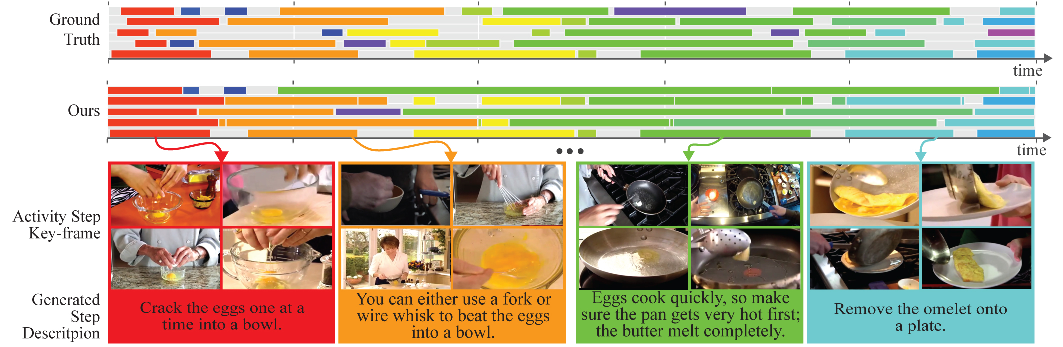
\includegraphics[width=\textwidth]{figure_8a_flattened}
  \end{subfigure}~
\caption{How to make an omelet?}
      \label{recipe:ommelette}
       \begin{subfigure}[b]{\textwidth}
    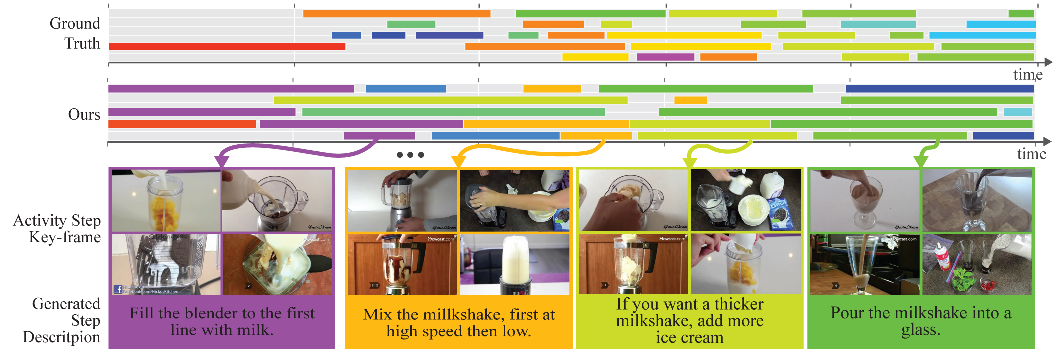
\includegraphics[width=\textwidth]{figure_8b_flattened}
  \end{subfigure}~
 \caption{How to make a milkshake?}
    \label{recipe:milkshake}
\caption{Temporal segmentation of the videos by our method and ground truth segmentation. We also color code the learned activity labels and visualize sample frames and the automatically generated captions for some of them. \emph{Best viewed in color.}}
\label{recipe:ommelette}
\fi
%\normalsize}
\end{figure*}

As shown in the Figures~\ref{recipe:ommelette}\&\ref{recipe:milkshake}, resulting steps are semantically meaningful. Moreover, the language captions are also quite informative hence we can conclude that there is enough language context within the subtitles in order to detect activities. On the other hand, some of the activity steps always occur together and our algorithm merges them into a single step while promoting sparsity.
\subsection{Quantitative Results}
\begin{figure*}[t]
  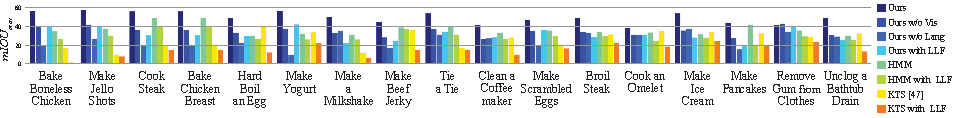
\includegraphics[width=\textwidth]{figure_9}
  \caption{$IOU_{max}$ values for all recipes, for all competing algorithms.}
  \label{mIOU}
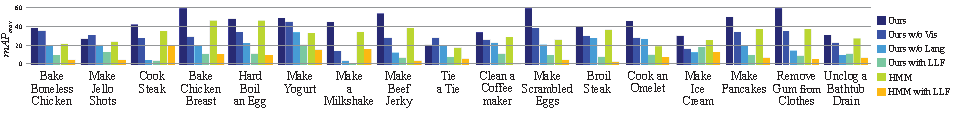
\includegraphics[width=\textwidth]{figure_10}
\caption{$AP_{max}$ values for all recipes, for all competing algorithms.}
\label{mmAP}
\end{figure*}

We compare our algorithm with the following baselines in the following sections.
\noindent\textbf{Low-level features (LLF):}
In order to experiment the effect of language and visual atom learning, we compare with low-level features in different algorithms. As a feature, we use HOG, HOF and MBH features and use frame-wise Fisher vector representation using the implementation of Oneata et al.\cite{fastLaptev}. As an observation model, we follow the Drichelet distribution since the Fisher vector is a histogram.

\noindent\textbf{Single modality:}
To experiment the importance of the effect of multi-modal approach, we also compare with single modality based approach whenever possible. We simply experiment based on a single modality.

\noindent\textbf{Hidden Markov Model (HMM):}
To experiment the effect of joint generaive model, we compare our algorithm with an HMM. We use the Baum-Welch algorithm\cite{rabiner} and choose the number of clusters via cross-validation.


\noindent\textbf{Kernel Temporal Segmentation\cite{potapov2014category}:}
Kernel Temporal Segmentation (KTS) proposed by Potapov et al.\cite{potapov2014category} can detect the temporal boundaries of the events/activities in the video from a time series data without any supervision. It enforces a local similarity of each resultant segment.

\subsubsection{Results}
Given a parsing result and a ground truth, we evaluate both quality of temporal segmentation and also the quality of the activity step discovery. 

We base our evaluation on two widely used metrics intersection over union and mean average precision. Intersection over union measures the quality of temporal segmentation and it is defined as; $IOU=\frac{1}{N}\sum_{i=1}^N \frac{\tau^\star_i \cap \tau^\prime_{i}}{\tau^\star_i \cup \tau^\prime_{i}}$ where $N$ is the number of segments, $\tau^\star_i$ is ground truth temporal segment and $\tau^\prime_{i}$ is the detected segment. Moreover, mean average precision is defined per activity part class and can be computed based on a precision-recall curve following TREC\cite{trecc} definition. Both of these metrics require the consistent labelling of ground truth and detection result, however, in an unsupervised setting the labels can be misaligned for example our algorithm can call activity step 1 of ground truth as activity step 3. The solution to this problem is a widely used cluster similarity measure(csm)\cite{liao05} which simply enables us using any metric in unsupervised setting. For any metric, it simply search over all possible matching between ground truth label and predicted label and choose the matching which gives the best result. Hence, we are using $mAP_{csm}$ and $IOU_{csm}$ as evaluation metrics.


\paragraph{Accuracy of the temporal parsing.}
In this section, we discuss the results presented in Figure~\ref{mIOU}. $IOU_{cms}$ captures the accuracy of the temporal segmentation of the videos. As shown in the Figure~\ref{mIOU}, proposed method consistently outperforms the competing algorithms and its variations. One interesting observation is the importance of both modalities as a result of dramatic difference between the accuracy of our method and its single modality version.

Moreover, the difference between our method and HMM is also significant. We believe this is because of the ill-posed definition of activities in HMM since the granularity of the activity steps is subjective. On the other hand, our method starts with the well-defined definition of finding set of steps which generate the entire collection. Hence, our algorithm do not suffer from granularity problem.

We also average over the metrics over recipes and include in the following table;
\begin{table}
\caption{Average of $IOU_{cms}$ and $mAP_{cms}$ over recipes.}
{\small
\resizebox{\columnwidth}{!}{%
\begin{tabular}{c|cc|cc|cccc}
 & KTS \cite{potapov2014category}    & KTS\cite{potapov2014category}     & HMM     & HMM    & Ours    & Ours     & Ours      & Our  \\
 &  w/ LLF &  w/ Sem &  w/ LLF &  w/Sem &  w/ LLF &  w/o Vis &  w/o Lang &  full \\
 \hline 
$IOU_{cms}$  & 16.80 & 28.01      & 30.84 &   37.69   &  33.16 &  36.50 & 29.91& 52.36 \\
$mAP_{cms}$  &  n/a  & n/a        & 9.35  &   32.30   &  11.33 &  30.50 &  19.50 & 44.09 \\
\end{tabular}}}
\normalsize
\end{table}

\paragraph{Coherency and accuracy of activity step discovery.}
Although $IOU_{cms}$ successfully measures the accuracy of the detected activities, it can not measure the matching activities over different videos since the metric is based on independent videos. Therefore, we are using $mAP_{cms}$ for measuring the accuracy of activity discovery over a video collection.

In order to further evaluate the role of semantics, we also performed a subjective analysis. Since, we have an evaluation set -ground truth activity labels-, we concatenated them into a label collection. Then, we collected the outputs of our algorithm, and the computing ones. We ask non-expert users to choose a label for each discovered activity. In other words, we replaced the maximization with subjective labelling. We designed our experiments in a way that each clip received annotations from 5 different users. Moreover, we randomized the ordering of videos and algorithms during the subjective evaluation. We compute the mean average precision and call it $mAP_{sem}$. We also only used 5 random recipes out of 25.

\begin{table}
\caption{Semantic mean-average-precision $mAP_{sem}$ computed based on subjective evaluation.}
{\small
\resizebox{\columnwidth}{!}{%
\begin{tabular}{c|cc|cccc}
            & HMM     & HMM    & Ours    & Ours     & Ours      & Our  \\
            & w/ LLF  &  w/Sem &  w/ LLF &  w/o Vis &  w/o Lang &  full \\ \hline
$mAP_{sem}$ & 6.44   & 24.83  &     7.28 &   28.93  &  14.83    &  39.01 \\
\end{tabular}}}
\normalsize
\end{table}
Both $mAP_{cms}$ and $mAP_{sem}$ metrics suggest that our method consistently outperforms the competing ones. There is only one recipe in which our method is outperformed by our based line of no visual information. This is mostly because of the specific nature of the recipe \emph{How to tie a tie?}. In such videos the notion of object is not useful since all videos use a single object over the entire video. This single object is a \emph{tie} and does not fit the assumption of a frame based on multiple visual atoms. 


\paragraph{How important is each modality?}
In order to experiment the importance of using both language and vision modalities, we compare our method with a self-baseline of using a single modality. As shown in Figure~\ref{mIOU} and \ref{mmAP}, our method significantly outperforms both of the baselines consistently in all recipes. Hence, we need to use both modalities. This result is expected because visual cues are good at separating different activities within the same video since the visual appearance is not changing much. However, language does not help much since there is too much background information other than the actual activity. On the other hand, language is good at relating activities from different videos since there is not much inter-class variation and it is easy to detect these variations caused by synonyms etc. thanks to the strong structure of the language modality. We believe this behaviour is the rationale behind the fact the language-only is slightly better.